In general, spectral smoothing may be applied to any function of frequency.
Here, we restrict our discussion to raw (i.e., not smoothed) frequency spectra whose data points are specified at uniformly-spaced frequencies on a linear scale, such as those obtained through an FFT.
Furthermore, in the applications of spectral smoothing mentioned in the introduction, the spectra to be smoothed are typically frequency or magnitude responses of acoustic transfer functions, rather than Fourier transforms or power spectra of time-domain signals.\footnote{This distinction becomes necessary when discussing interpolation to a log-frequency scale.
For example, for power spectra of time-domain signals, conversion from a linear frequency scale to a log-frequency scale should also involve a change of units of the vertical axis, such that the values that are plotted on a linear frequency scale represent power per unit linear frequency, whereas those plotted on a log-frequency scale represent power per unit log-frequency.
Through this conversion, a pink-noise power spectrum plotted over linear frequency would exhibit the usual $-3$~dB/octave slope, while on a log-scale, the spectrum would appear flat.
Consequently, on either frequency scale, integrating the power spectrum over a given frequency band gives the total power in that band.
However, for frequency (or magnitude) responses of transfer functions, the values that are plotted are gains for specific frequencies, regardless of the distribution of those frequency points.
Consequently, interpolation of a frequency response to a log-frequency scale should involve only a ``resampling'' of the response to logarithmically-spaced frequencies; it should not involve a change of units.} Consequently, we further restrict our discussion to the smoothing of frequency or magnitude responses of transfer functions.

Consider a raw, possibly complex-valued frequency spectrum of length $N$ denoted by $X[k]$, where $k$ is the discrete frequency index.
The smoothed spectrum is given by
\begin{equation}\label{eq:A3_Smoothing_Weights:SmoothingSummation}
X_\textrm{s}[k] = \sum_{k' = 0}^{N - 1} W[k, k'] X[k']
\end{equation}
for all integers $k,k' \in [0, N - 1]$, where, for a given value of $k$, $W[k, k']$ denotes the $k^{\textrm{th}}$ sequence of non-negative weights used to smooth the raw spectrum \citep{HatziantoniouMourjopoulos2000}.
These weights are normalized such that, for all $k \in [0, N - 1]$,
\begin{equation}\label{eq:A3_Smoothing_Weights:WeightNorm}
\sum_{k' = 0}^{N - 1} W[k, k'] = 1.
\end{equation}

The smoothing operation defined by \eqnref{eq:A3_Smoothing_Weights:SmoothingSummation} can be thought of as a frequency-domain convolution with a frequency-dependent kernel, $W[k, k']$.
In the case of a frequency-invariant smoothing window (e.g., a fixed-width moving-average filter), we can instead define a single weight sequence $W[k - k'] = W[k, k']$, and \eqnref{eq:A3_Smoothing_Weights:SmoothingSummation} takes the standard form of convolution.

To compute the smoothed spectrum at a given frequency $f = k F_s / N$, where $F_s$ is the sampling rate, the (exact) lower and upper cutoff frequencies of the weighting function are given by
\begin{equation}\label{eq:A3_Smoothing_Weights:cutoffs}
    \begin{array}{ll}
    f_L &= f \cdot 2^{-\Delta/2},\\[8pt]
    f_U &= f \cdot 2^{+\Delta/2},
    \end{array}
\end{equation}
respectively \citep{HatziantoniouMourjopoulos2000}, where $\Delta$ is the smoothing bandwidth in octaves.
Consequently, the ratio, $Q$, of the center frequency to the bandwidth is a constant, and its reciprocal is given by
\begin{equation}\label{eq:A3_Smoothing_Weights:QFactor}
\frac{1}{Q} = \frac{f_U-f_L}{f} = 2 \sinh \left( \frac{\Delta \log (2)}{2} \right).
\end{equation}

%%%% Hatziantoniou's Method %%%%
\subsection{Method 1: symmetric weights} \label{sec:A3_Smoothing_Weights:Smoothing_Methods:Hatziantoniou_Method}
In the method presented by~\citet{HatziantoniouMourjopoulos2000}, the smoothed spectrum is computed using~\eqnref{eq:A3_Smoothing_Weights:SmoothingSummation}, where the weighting function is derived by first defining the half-length of the $k^{\textrm{th}}$ weight sequence as
\begin{equation}\label{eq:A3_Smoothing_Weights:HatzHalfWidth}
m[k] = \left\lfloor \frac{1}{2}\frac{k}{Q} \right\rfloor,
\end{equation}
where $\lfloor \cdot \rfloor$ denotes rounding down to the nearest integer.
The weighting function for a rectangular window is then given by
\begin{equation}\label{eq:A3_Smoothing_Weights:HatzWeights}
W_{\textrm{R}}[k, k'] = \left\{
    \begin{array}{cl}
	\displaystyle \frac{1}{2 m[k] + 1} & \textrm{for } \left| k - k' \right| \leq m[k],\\[8pt]
	0 & \textrm{for } \left| k - k' \right| > m[k].
    \end{array}\right.
\end{equation}
From this definition we see that each weight sequence is a rectangular window with $2 m[k] + 1$ non-zero values centered around $k = k'$.
This is in conflict with~\eqnref{eq:A3_Smoothing_Weights:cutoffs}, as the upper cutoff frequency should be further from the center than the lower cutoff, but instead the two ends of the weight sequence are equidistant to the center.
As we will show in~\secref{sec:A3_Smoothing_Weights:Analysis}, this error becomes significant for large smoothing bandwidths.

%%%% Lipshitz' Method %%%%
\subsection{Method 2: interpolation to logarithmic scale} \label{sec:A3_Smoothing_Weights:Smoothing_Methods:Lipshitz_Method}
In the method proposed by~\citet{Lipshitz1985}, the raw spectrum is first interpolated to a logarithmic frequency scale, at which point a fixed-width moving-average filter is applied.
The authors suggest interpolating to $N/2$ logarithmically-spaced frequencies, which we denote $\kappa[\ell]$, given by
\begin{equation}
\kappa[\ell] = \left( \frac{N}{2} \right)^\frac{\ell}{N/2-1},
\end{equation}
such that $1 \leq \kappa[\ell] \leq N/2$ for all integers $\ell \in [0, N/2 - 1]$.
The interval in octaves between any two adjacent frequencies is a constant, given by
\begin{equation}
\beta = \log_2 \frac{\kappa[\ell + 1]}{\kappa[\ell]} = \frac{1}{N/2-1} \log_2 \frac{N}{2},
\end{equation}
and, as we did for method 1, we define the weight-sequence half-length, $\mu$, as
\begin{equation}
\mu = \left\lfloor \frac{\Delta/2}{\beta} \right\rfloor,
\end{equation}
which is also constant.

To perform the interpolation,~\citet{Lipshitz1985} suggest a 4-point polynomial (i.e., cubic) interpolation, but, in general, any interpolation scheme (e.g., linear, spline, etc.) may be employed.
Here, we use linear interpolation, such that the interpolated raw spectrum, $\hat{X}$, which is now a function of the log-frequency index $\ell$, is given by
\begin{equation}\label{eq:A3_Smoothing_Weights:LogInterpolate}
\hat{X}[\ell] = X[k_1] + \left( X[k_2] - X[k_1] \right) \frac{\kappa[\ell] - k_1}{k_2 - k_1},
\end{equation}
where $k_1 = \big\lfloor \kappa[\ell] \big\rfloor$ and $k_2 = k_1 + 1$.

The smoothed spectrum, $\hat{X_\textrm{s}}$, is also a function of $\ell$ and is given by
\begin{equation}
\hat{X_\textrm{s}}[\ell] = \sum_{\ell' = 0}^{N/2 - 1} \hat{W}[\ell - \ell'] \hat{X}[\ell'],
\end{equation}
where $\hat{W}$ is the weighting function.
For a rectangular window, $\hat{W}$ is given by
\begin{equation}
\hat{W}_{\textrm{R}}[\ell - \ell'] = \left\{
    \begin{array}{cl}
	\displaystyle \frac{1}{2 \mu + 1} & \textrm{for } \left| \ell - \ell' \right| \leq \mu,\\[8pt]
	0 & \textrm{for } \left| \ell - \ell' \right| > \mu.
    \end{array}\right.
\end{equation}
The smoothed spectrum is then interpolated back to a linear frequency scale by
\begin{equation}
X_\textrm{s}[k] = \hat{X_\textrm{s}}[\ell_1] + \left( \hat{X_\textrm{s}}[\ell_2] - \hat{X_\textrm{s}}[\ell_1] \right) \frac{k - \kappa[\ell_1]}{\kappa[\ell_2] - \kappa[\ell_1]},
\end{equation}
where $\ell_1 = \left\lfloor (N/2 - 1) \log_{N/2} (k) \right\rfloor$ and $\ell_2 = \ell_1 + 1$.

%%%% Proposed Method %%%%
\subsection{Method 3: logarithmically-compensated weights} \label{sec:A3_Smoothing_Weights:Smoothing_Methods:Proposed_Method}
Consider a window $w(\phi)$ that is a function of the continuous variable $\phi$ (we will see later that $\phi$ is related to frequency).
Let $w$ be an even function of $\phi$ whose total integral is unity, i.e.,
\begin{equation}\label{eq:A3_Smoothing_Weights:WindowNorm}
\int_{-\infty}^{\infty} w(\phi) d\phi = 1.
\end{equation}

For example, given a smoothing bandwidth of $\Delta$ octaves, the normalized rectangular window is given by
\begin{equation}\label{eq:A3_Smoothing_Weights:RectangularWindowLogf}
w_\textrm{R}(\phi) = \left\{
    \begin{array}{cl}
	1/\Delta & \textrm{for } |\phi| \leq \Delta/2,\\[8pt]
	0 & \textrm{for } |\phi| > \Delta/2.
    \end{array}\right.
\end{equation}

For a given center-frequency index, $k$, we compute the weighting function by successively integrating adjacent slices of the window function, i.e.,
\begin{equation}\label{eq:A3_Smoothing_Weights:WeightsIntegral}
W[k, k'] = \int_{\Phi[k, k' - 0.5]}^{\Phi[k, k' + 0.5]} w(\phi) d\phi
\end{equation}
for all integers $k,k' \in [0, N - 1]$, where $\phi$ represents log-frequency in octaves relative to $k$, i.e., $\log_2(k'/k)$, and the limits of integration are given by
\begin{equation}\label{eq:A3_Smoothing_Weights:WeightsIntegralLimits}
\Phi[k, k' \pm 0.5] = \log_2 \left( \frac{k' \pm 0.5}{k} \right).
\end{equation}
As for method 1, the smoothed spectrum is then computed using~\eqnref{eq:A3_Smoothing_Weights:SmoothingSummation} but with this new weighting function.
Due to the normalization of the window function imposed in~\eqnref{eq:A3_Smoothing_Weights:WindowNorm}, each resulting weight sequence is also normalized and satisfies~\eqnref{eq:A3_Smoothing_Weights:WeightNorm}.

%% Example %%
%\begin{example*}
\paragraph*{Example:} To illustrate the difference between the calculated weights and the window function, consider the weight sequence needed to compute the value of the smoothed spectrum at $k = 10$, for 1-octave smoothing.
The window function is given by \eqnref{eq:A3_Smoothing_Weights:RectangularWindowLogf}, and the weights will be non-zero for, at most, $\lfloor k \cdot 2^{-\Delta/2} \rfloor \leq k' \leq \lceil k \cdot 2^{+\Delta/2} \rceil$, i.e., $k' \in [7, 15]$, where $\lceil \cdot \rceil$ denotes rounding up to the nearest integer and the bounds of the inequalities are obtained by substituting $k$ for $f$ in~\eqnref{eq:A3_Smoothing_Weights:cutoffs}.
However, integrating the window function for all slices reveals that $W[10,15] = 0$, since that integral begins at $\log_2 (14.5/10)$ but the window function already dropped to zero at $\phi \approx \log_2 (14.142/10)$.

\begin{figure}[t]
    \centering
    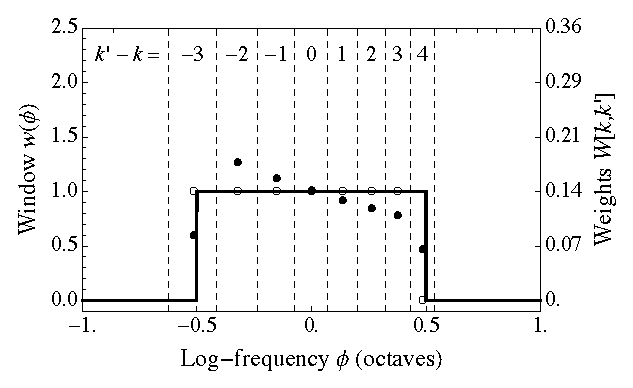
\includegraphics[width=0.6\columnwidth]{a3_smoothing_weights/figures/RectangularWeightsExample.eps}
    \caption[Calculated smoothing weights for a rectangular window function.]{
    Calculated weighting function $W[k,k']$ for methods 1 (symmetric weights -- empty circles) and 3 (log-compensated weights -- filled circles) for a rectangular window function $w(\phi)$ (solid curve).
In this example, $k = 10$ and $\Delta = 1$~octave.
Dashed vertical lines (and ticks on the top axis) indicate the limits of integration, $\Phi[10, k' \pm 0.5]$, given by \eqnref{eq:A3_Smoothing_Weights:WeightsIntegralLimits}.}
    \label{fig:A3_Smoothing_Weights:RectangularWeightsExample}
\end{figure}

The calculated non-zero weights are shown as filled circles in \figref{fig:A3_Smoothing_Weights:RectangularWeightsExample} along with the window function, both as functions of $\phi$.
From this plot, we observe two features of the weight sequence.
First, the end points take into account the extent to which the window function occupies the corresponding frequency interval, whereas simply evaluating the window function at each $k'$ would only ever give either 0 or $1/\Delta$.
Second, the intermediate points exhibit a frequency-dependent trend similar to that of a pink-noise power spectrum.
Indeed, this sequence is derived to assign equal weight per unit log-frequency (e.g., octave), so although the width of each frequency interval is constant, the ratio between the upper and lower edges of the interval decreases with increasing frequency, so the weight must also decrease.

For comparison, the weights for method 1 are also shown in \figref{fig:A3_Smoothing_Weights:RectangularWeightsExample} as empty circles that remain constant ($W[k,k'] = 1/7$) for $| k - k' | \leq m[k] = 3$ and zero otherwise.
%\end{example*}